\documentclass{article}

\usepackage{graphicx}
\usepackage[utf8]{inputenc}
\usepackage[english]{babel}
\usepackage[document]{ragged2e}



\begin{document}

\textbf{Q3}  
\textbf{Edge-preserving Smoothing using Patch-Based Filtering.}
\vskip 0.2in

Pranav Sankhe \texttt{150070009} \newline
Kalpesh Krishna \texttt{140070017}  \newline
Mohit Madan \texttt{15D070028} \newline

\vskip 0.5in

\textbf{Report:}  
\vskip 0.1in
Resized the image by subsampling by a factor of 2 along each dimension, after applying a Gaussian blur of standard deviation around 0.66 pixel width. \newline

\texttt{Window Size = 25*25}   \newline
\texttt{Patch size = 9*9}  \newline

Here are the results for \texttt{sigmaSpatial = 1.4} and \texttt{sigmaIntensity = 1.08}: 

\begin{figure}[h!]
  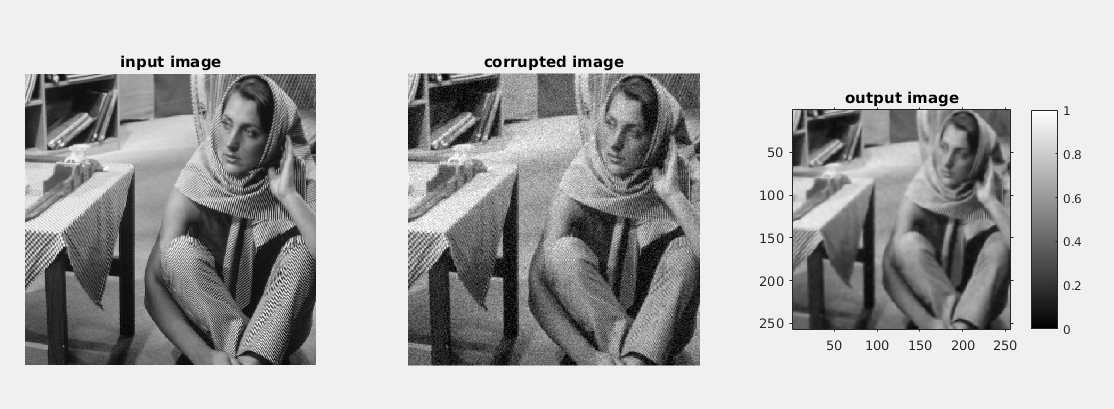
\includegraphics[width=\linewidth]{result.png}
  \caption{Original,corrupted and filtered images.}
  \label{fig:result1}
\end{figure}


\begin{figure}[h!]
  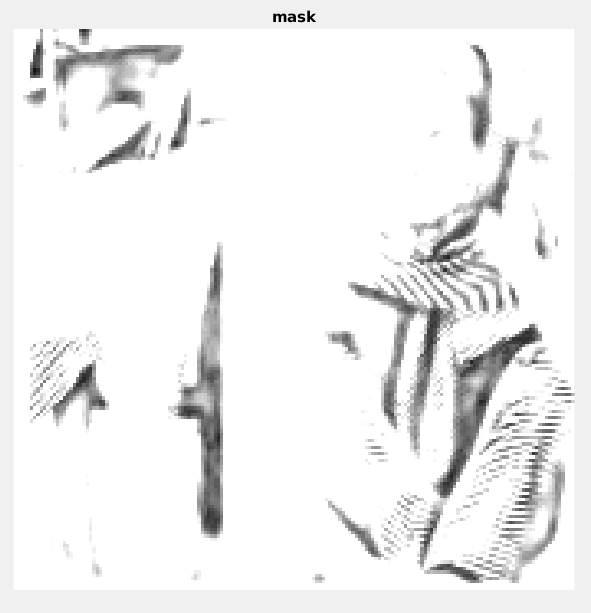
\includegraphics[width=\linewidth]{mask.png}
  \caption{Mask used to make patches isotropic.}
  \label{fig:result2}
\end{figure}

\newpage
\textbf{Optimal parameter} values are as follows: \newline
\texttt{sigmaSpatial = 1.4} \newline
\texttt{sigmaIntensity = 1.08} \newline  
\texttt{RMSD} for the optimal parameter is 0.0394

\vskip 0.2in

\texttt{RMSD} for \(1.1*\sigma = 0.406\) \newline
\texttt{RMSD} for \(0.9*\sigma = 0.145\) 

%\texttt{RMSD} for 0.9*\sigma = 0.145






\end{document}